\section{Clustering}
\label{sec:clustering}
In this part we explore an in-depth comparison of different clustering algorithms, such as K-Means, DBSCAN, Hierarchical. Then a small parenthesis is opened on other options such as the Expectation-maximization algorithm, X-Means and Fuzzy C-Means.

\subsection{Features selection}
At the beginnig of our research we tried to find a pattern that could relate the style of the player ( \textit{rel ace},  \textit{rel df},  \textit{rel 1stIn},  \textit{rel 1stWon},  \textit{rel 2ndWon}) with respect to his strength. After feature engineering, clustering and analysis we found no meaningful results. So, we decide to switch to the analysis that we will present in this report.
\\We have decided to select the features respecting the following criteria in order
\begin{itemize}
	\item Selection of those features that may provide an interesting picture about the performance of the players.
	\item Dropped all the couple of features that have more than `70\%` of correlation. Leaving just one feature per correlated pair.
	\item Removed features deemed unimportant that had a good percentage of null values.
\end{itemize}

% Since in the player's dataframe there was a big number of records with NaN values, corresponding to the in-match statistics (rel\_ace, rel\_df, rel\_1stIn etc.), we set a threshold establishing that every player in order to be in the dataframe should have played at list 15 matches with non-null values for these features.
% Then we selected the features which seemed to better represent the “strength” of a player, and we performed the correlation analysis (Fig. \ref{fig:correlation_plot}) in order to have a narrower selection. Whenever two features had a correlation greater than 70\% (Pearson coefficient), we discarded one of the two. 
As a results we obtained the following uncorrelated features:
\begin{center}
	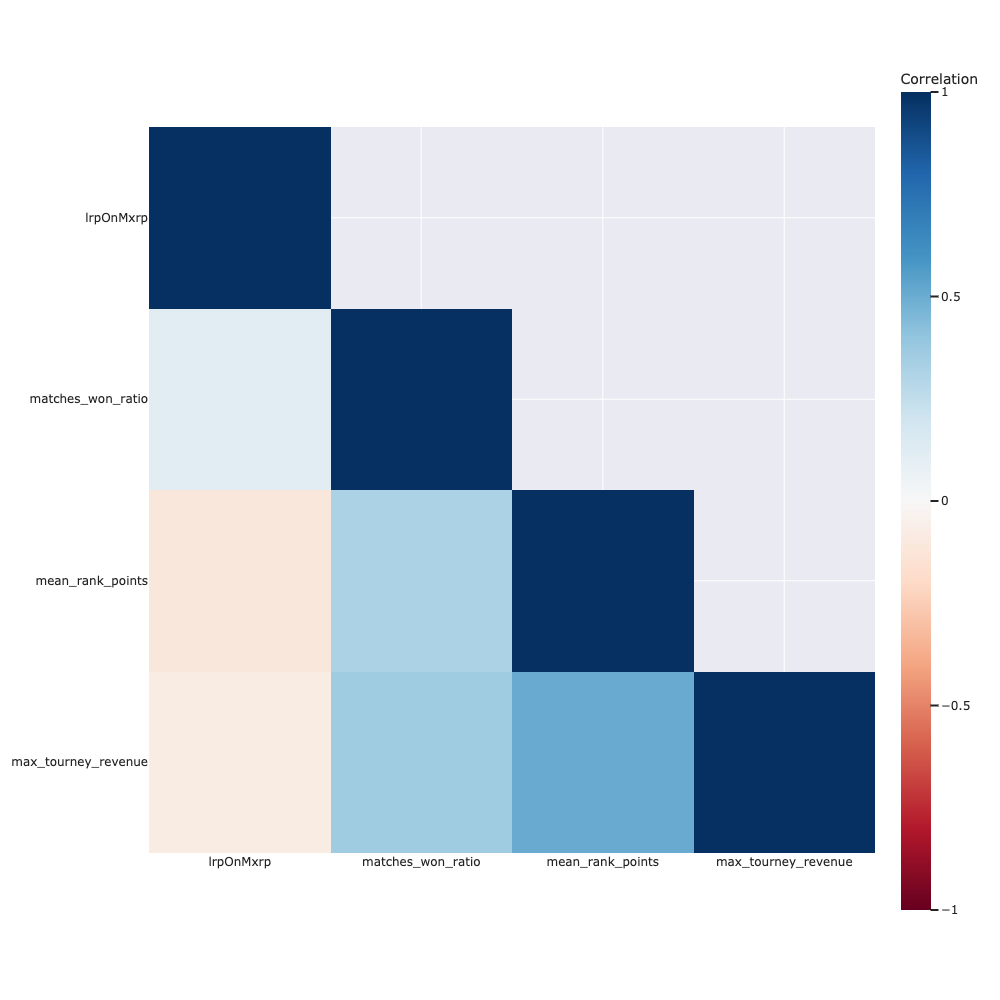
\includegraphics[width=280px]{plots/correlation_plot}
	\label{fig:correlation_plot}
	\captionof{figure}{Correlation Plot}\label{fig1}
\end{center}
At this point the remaining features were: '\textit{lrpOnMxrp}', '\textit{matches\_won\_ratio}', '\textit{mean\_rank\_points}',\\ '\textit{max\_tourney\_revenue}'.\\
Those features will be used as a starting point in the clustering.

\subsection{Pre-processing}
In order to prepare the data for the clustering, we performed a normalization of the data with MinMaxScaler in order to assign the same weight to each clustered feature.
The number of players used to cluster is equal to 2997.

\subsection{K-means}
\label{sec:k-means}
% \subsubsection{Distributions and preprocessing}
% Being K-means suitable for globular cluster, we decided to perform logarithm to the \textit{mean\_rank\_points} feature that follow a power law to lead to a more compact distribution:
% \ref{fig:mean_rank_points}  \ref{fig:log_mean_rank_points}.

% \begin{figure}[h]
% \centering
% \begin{minipage}{.5\textwidth}
% \centering
% 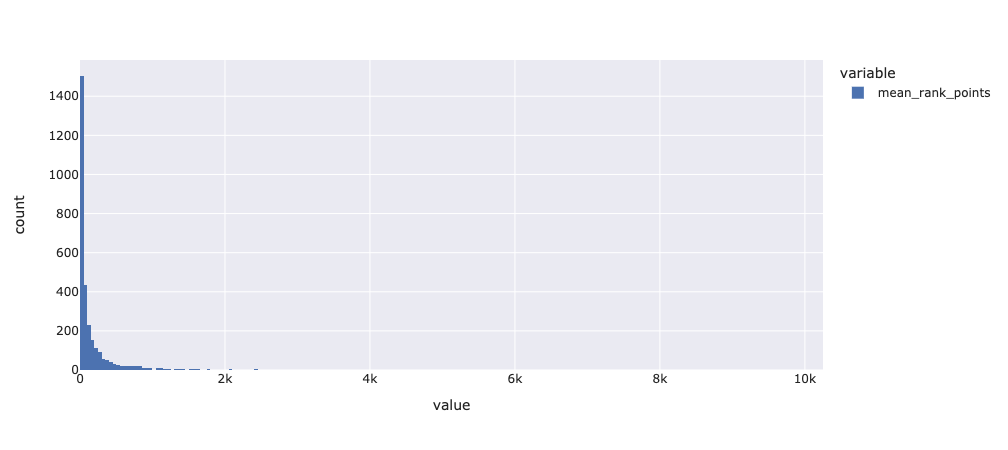
\includegraphics[width=\textwidth]{plots/kmeans/preprocessing/mean_rank_points}
% \captionof{figure}{Mean rank points}
% \label{fig:mean_rank_points}
% \end{minipage}%
% \begin{minipage}{.5\textwidth}
% \centering
% 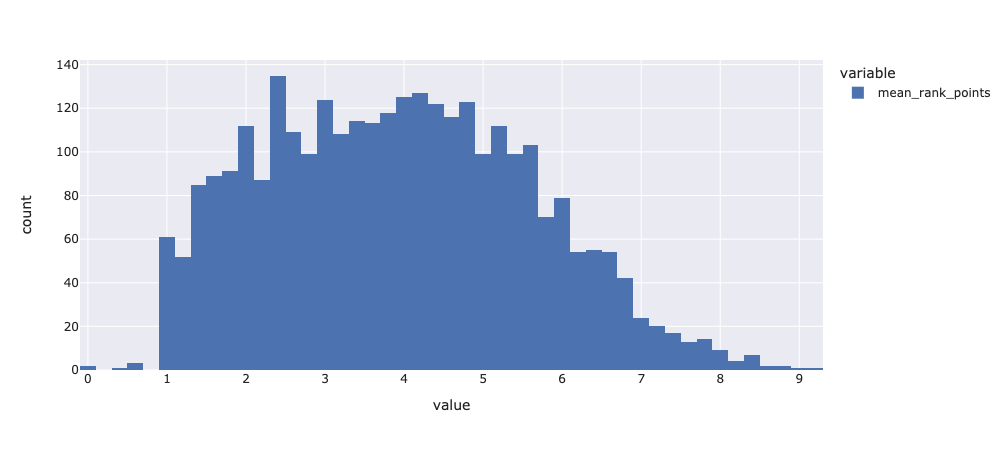
\includegraphics[width=\textwidth]{plots/kmeans/preprocessing/log_mean_rank_points.png}
% \captionof{figure}{Variance rank points}
% \label{fig:log_mean_rank_points}
% \end{minipage}
% \end{figure}
The first step was to find the \textbf{optimal K}. It was done by following the elbow rule, that suggested to use $k=4$ where the SSE score was 151.183 (Fig. \ref{fig:kmeans_elbow_rule}). On the other hand, even the Silhouette score had the maximum value with $k=4$ (Fig. \ref{fig:kmeans_silhouette_score}), hence it was trivial to decide that the optimal $k$ overall was $k=4$. Moreover, the Silhouette score per cluster is represented in Fig. \ref{fig:kmeans_silhouette_average} and each cluster is balanced enough. Cluster 1 is the only one where a tiny amount of points has a negative score. Nonetheless, the overall balance is extremely good, because there is no presence of clusters with a silhouette score below the average and there are no wide fluctuations in the size of the silhouette plots.

\begin{figure}[!htb]
	\centering
	\begin{minipage}{.32\textwidth}
		\centering
		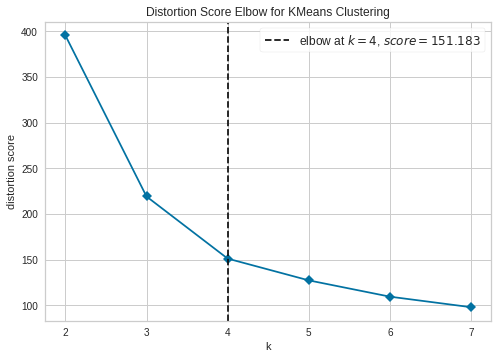
\includegraphics[width=\linewidth]{plots/kmeans/kmeans_elbow_rule}
		\captionof{figure}{Elbow rule}
		\label{fig:kmeans_elbow_rule}
	\end{minipage}%
	\begin{minipage}{.32\textwidth}
		\centering
		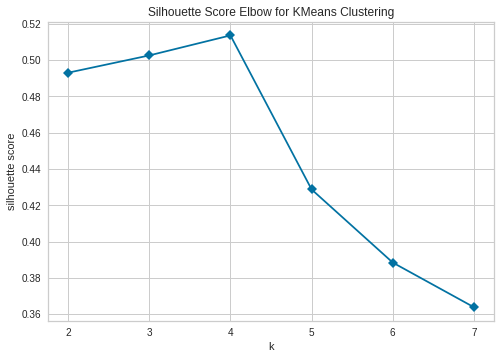
\includegraphics[width=\linewidth]{plots/kmeans/kmeans_silhouette_score}
		\captionof{figure}{Silhouette score}
		\label{fig:kmeans_silhouette_score}
	\end{minipage}
	\begin{minipage}{.32\textwidth}
		\centering
		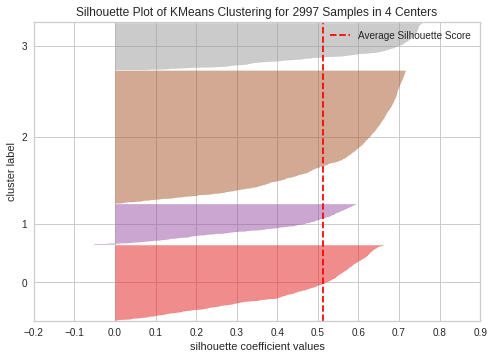
\includegraphics[width=\linewidth]{plots/kmeans/kmeans_silhouette_average}
		\captionof{figure}{Silhouette score average}
		\label{fig:kmeans_silhouette_average}
	\end{minipage}
\end{figure}

\subsubsection{Results interpretation}
\begin{figure}[!h]
	\centering
	\begin{minipage}{.45\textwidth}
		\centering
		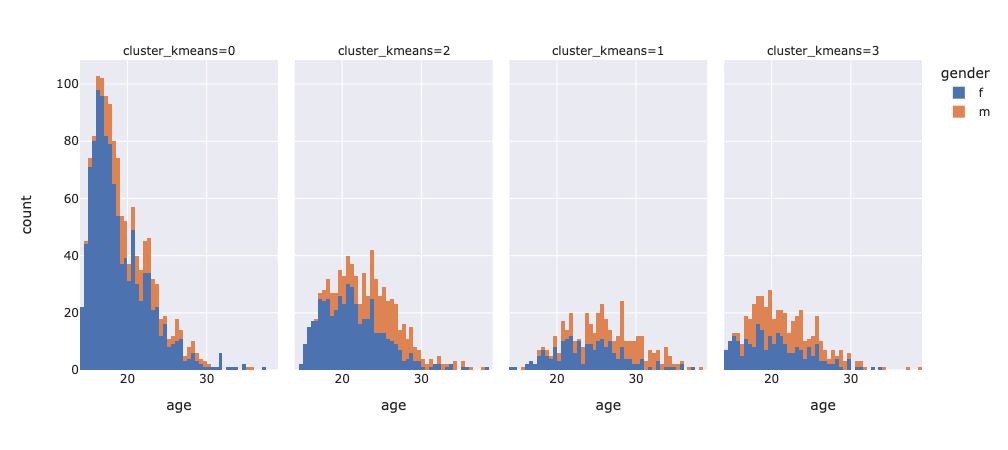
\includegraphics[width=\textwidth]{plots/kmeans/hist_age.png}
		\subcaptionof{(a) histogram of age for male/female}
		\label{fig:age_kmeans}
	\end{minipage}%
	\begin{minipage}{.45\textwidth}
		\centering
		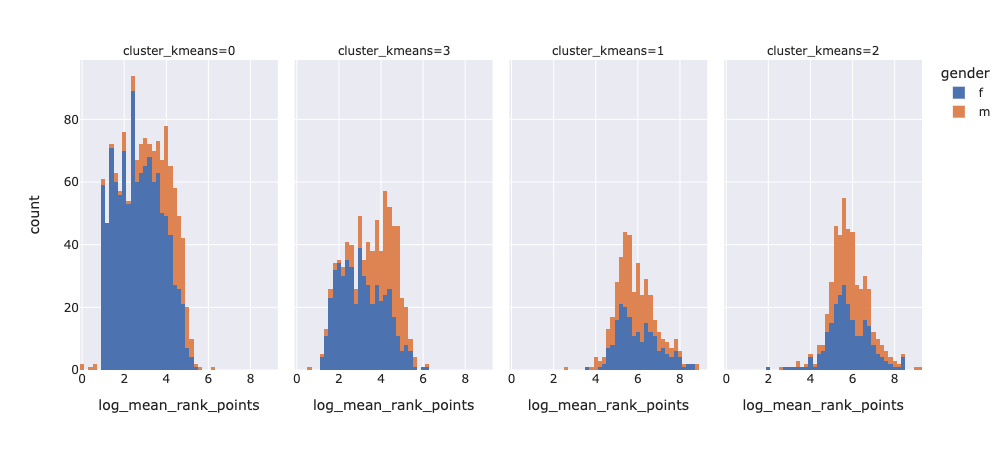
\includegraphics[width=\textwidth]{plots/kmeans/hist_log_mean_rank_points.png}
		\subcaptionof{(b) histogram of mean rank points for male/female}
		\label{fig:mean_rank_points_kmeans}
	\end{minipage}
	\begin{minipage}{.45\textwidth}
		\centering
		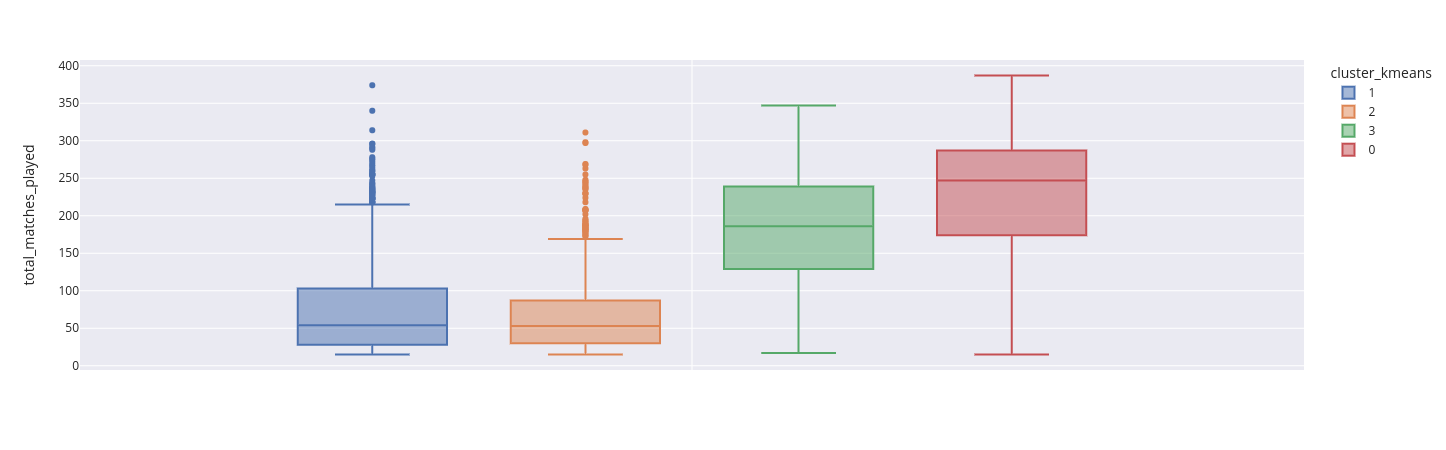
\includegraphics[width=\textwidth]{plots/kmeans/kmeans-box-plot-matches-played.png}
		\subcaptionof{(c) box plot of total matches played}
		\label{fig:total_match_played_kmeans}
	\end{minipage}%
	\begin{minipage}{.45\textwidth}
		\centering
		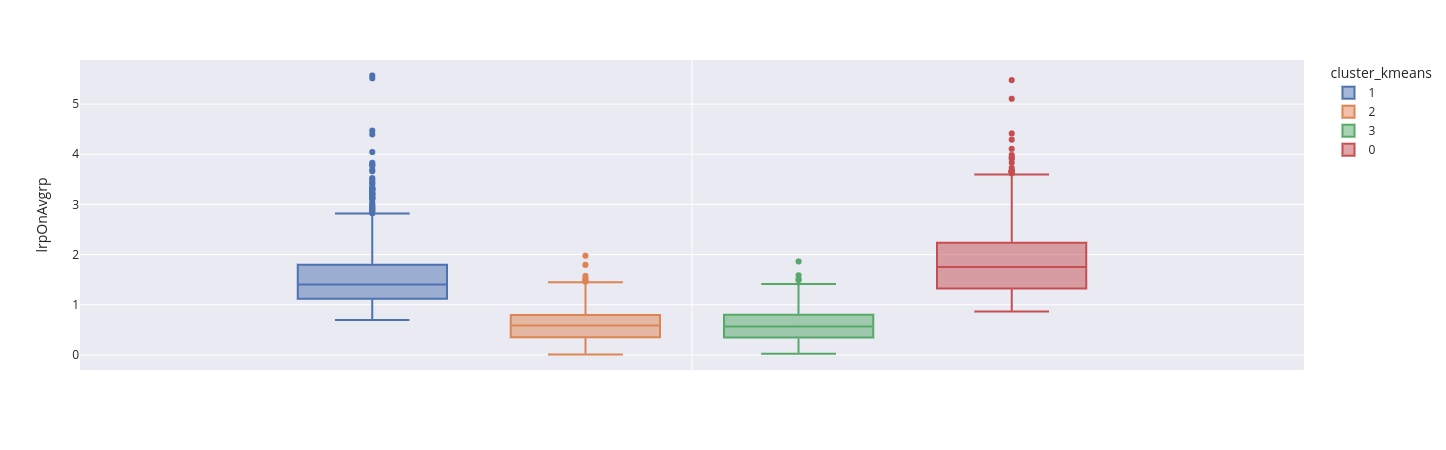
\includegraphics[width=\textwidth]{plots/kmeans/kmeans-box-plot-lrponavgrp.png}
		\subcaptionof{(d) box plot of last rank points on average rank points}
		\label{fig:lrpOnAvgrp_kmeans}
	\end{minipage}
	\captionof{figure}{Distributions of features within the dataset}
	\label{fig:kmeans_distributions}
\end{figure}
The clustering algorithm manages to find interesting groupings. Analysing Figure \ref{fig:kmeans_distributions} (a), it can be seen that cluster 0 has a lower average age and cluster 1 a higher one. 
On the other hand, in Figure \ref{fig:kmeans_distributions} (b) you can see a clearer division compared to the case described above and this is also due to the fact that it was used for clustering. Clusters 0 and 3 have lower average rank points than the two clusters. In addition, one can appreciate how the clustering found an extremely similar grouping regardless of gender, and this is also true for the other features that are not represented in this report but can be found in the attached Jupyter notebook.
In Figure \ref{fig:kmeans_distributions} (c), instead, a clear division can be seen in terms of the experience accumulated by the players; in clusters 1 and 2 the number of games played is on average lower than in the other two clusters. 
Finally, in Figure Image \ref{fig:kmeans_distributions} (d), we can appreciate the grouping by last rank points on average, which expresses the trend of the performance and cluster 0 and 1 have an average value that expresses an improvement, while the other two a worsening performance.
\\
The interpretation we gave to the results came from looking at the graph of centroids (Fig. \ref{fig:kmeans_centroid}) and looking at external features not used in the algorithm that seemed relevant, resulting in the following:
\begin{itemize}
	\item{ \textbf{Cluster 0} represents the \textbf{young promises} (45.04\%): those with low mean\_rank\_points with an increasing average trend of growth. They have the lowest age and a low experience.}
	\item{ \textbf{Cluster 1} represent the \textbf{old glories} (13.64\%): those with good rank points with a decreasing performance. They are the oldest and with a high experience.}
	\item{ \textbf{Cluster 2} represents the \textbf{good players} (15.81\%): those with good rank points with an increasing performance. They have an average age and with a high experience.}
	\item{ \textbf{Cluster 3} represents the \textbf{bad players} (25.49\%): with low rank points and a decreasing trend of growth. They have an average age and low experience.}
\end{itemize}
\begin{figure}[h]
	\centering
	\begin{minipage}{.50\textwidth}
		\centering
		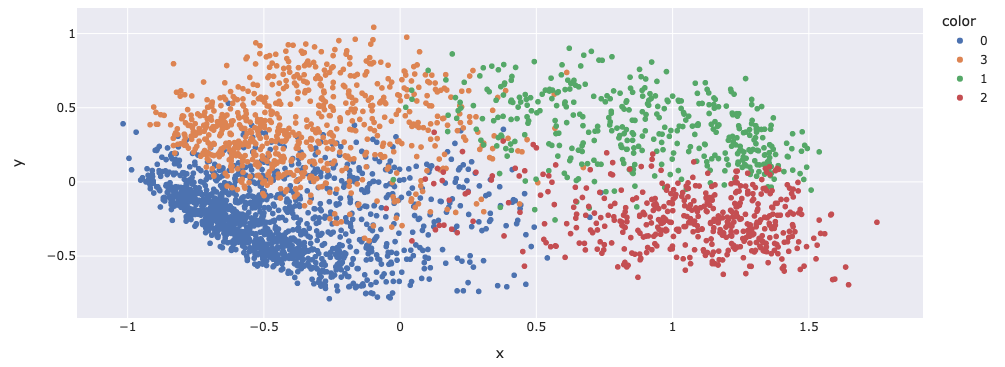
\includegraphics[width=\textwidth]{plots/kmeans/scatter_pca.png}
		\captionof{figure}{PCA visualization}
		\label{fig:pca_visualization}
	\end{minipage}%
	\begin{minipage}{.50\textwidth}
		\centering
		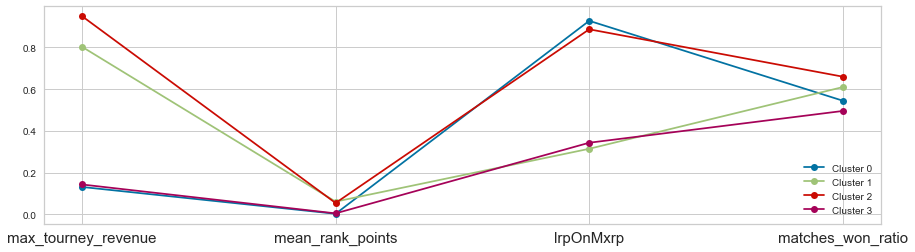
\includegraphics[width=\textwidth]{plots/kmeans/centers_plot.png}
		\captionof{figure}{Plotting k-means centroids}
		\label{fig:kmeans_centroid}
	\end{minipage}
\end{figure}
In Figure \ref{fig:pca_visualization} we compute the Principal Component Analysis related to the whole feature of the dataset, and we plot with respect to the two greater components, here we can depict the good separation among the clusters that the k-means performed.

\subsection{Density based}
The set of feature used for DBSCAN is the same as K-means, as well as for the applied transformations.\\
To understand a good range of values for the \verb|eps| parameter, we print the plot in Figure \ref{fig:dbscan_distances} to check the distances between the k-th nearest values for each possible point. Each distance is plotted in the x-axis, ordered with respect to the k-th nearest value.
\begin{figure}[h]
	\centering
	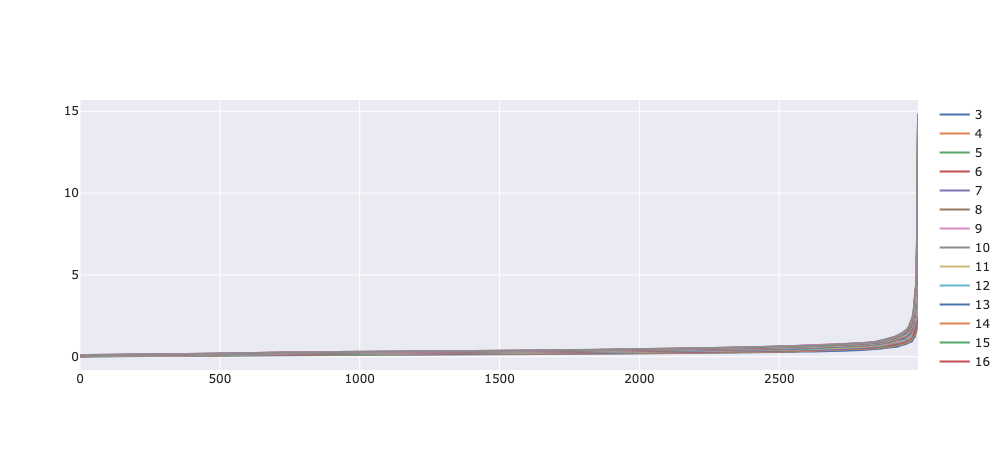
\includegraphics[width=\textwidth]{plots/dbscan/dbscan_distances}
	\captionof{figure}{Noise points with the k-th nearest neighbor at farther distance}
	\label{fig:dbscan_distances}
\end{figure}

Then, in order to find the proper parameters, we run a \textbf{grid-search} (Fig. \ref{fig:dbscan_metrics}) using a range of values for $eps=[0.1, 0.3]$. We also calculated the silhouette score, although it is not the best metric for DBSCAN it did allow us to make a decision and choose between different parameters. The rationale behind the choice of parameters was the following. Looking at the graph, we see that for large values of \verb|eps|, all points belong to one and only one cluster. For very small values, either the number of clusters is very large or all points are classified as noise. In addition, to reduce the options even further, probably it makes sense to consider number of clusters ranging from 2 to 4, hence $0.01 < eps < 0.25$. Finally, we took a high mean noise point distance to make sure that no dense clusters of noise formed, and at the same time for equal values we considered those values with a higher silhouette score. At this point, trying different combinations of parameters, one of the best choice was $eps=0.2, n=6$, to ensure a small number of outliers. With different parameters, either the number of outliers increased or clusters with a dozen elements were formed. In the next section, we comment on the results.

%  \ref{fig:dbscan_metrics}. Through the grid search in combination with the k-th distance plot (\ref{fig:dbscan_distances}) , we could get a better understanding of the kind of results we could expect for each rank and the resulting number of clusters.

\begin{figure}[h]
	\centering
	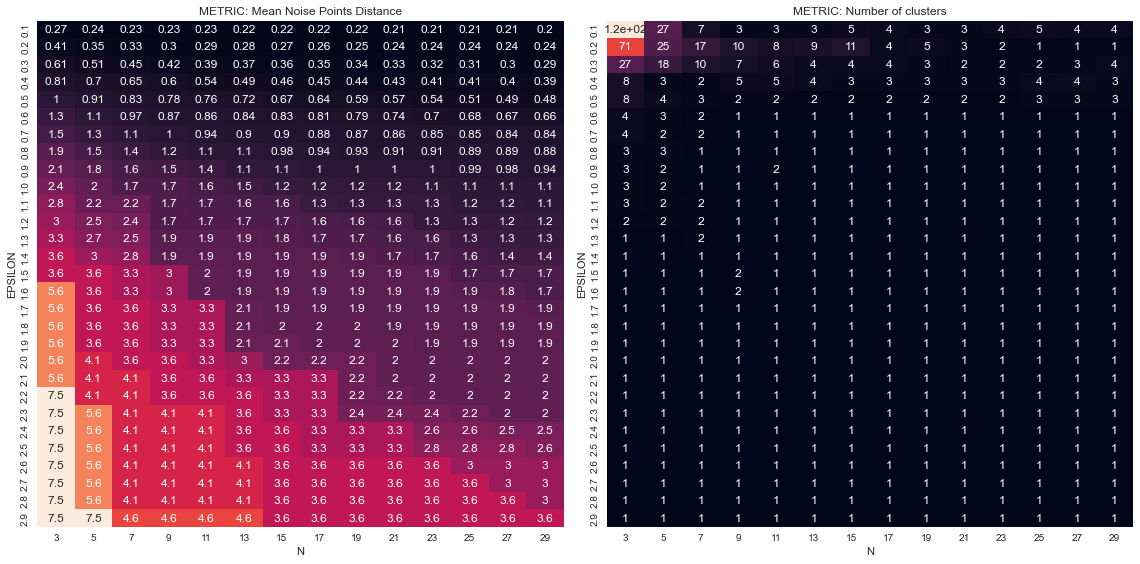
\includegraphics[width=\textwidth]{plots/dbscan/dbscan_metrics}
	\captionof{figure}{Chosen hyper-parameters $eps=0.2$ and $n=6$}
	\label{fig:dbscan_metrics}
\end{figure}

\subsubsection{Results interpretation}
The DBSCAN identified two clusters that are extremely heterogeneous and produced the following results which can be seen in Figure \ref{fig:dbscan_pca}, where the PCA visualization is shown, while in Figure \ref{fig:dbscan_scatter} where one can see a Pareto distribution, where 80\% of the players are poor and 20\% are good. In more detail, the results can be interpreted as follows:

\begin{figure}[h]
	\centering
	\begin{minipage}{.43\textwidth}
		\centering
		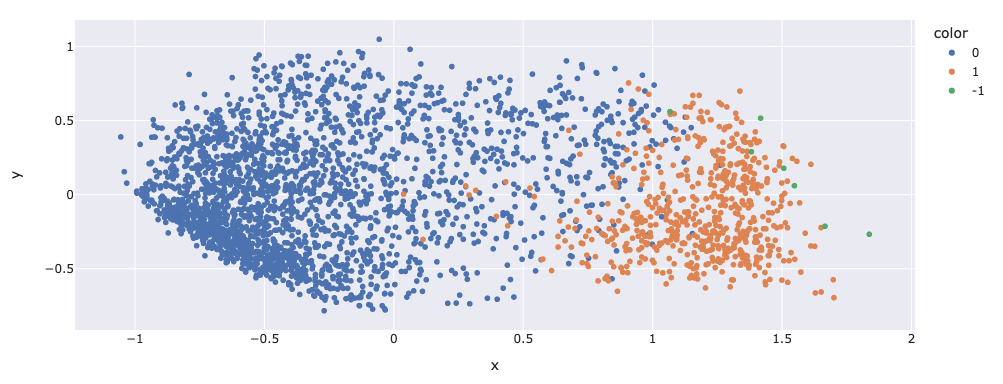
\includegraphics[width=\textwidth]{plots/dbscan/dbscan_pca.png}
		\captionof{figure}{PCA visualization}
		\label{fig:dbscan_pca}
	\end{minipage}%
	\begin{minipage}{.57\textwidth}
		\centering
		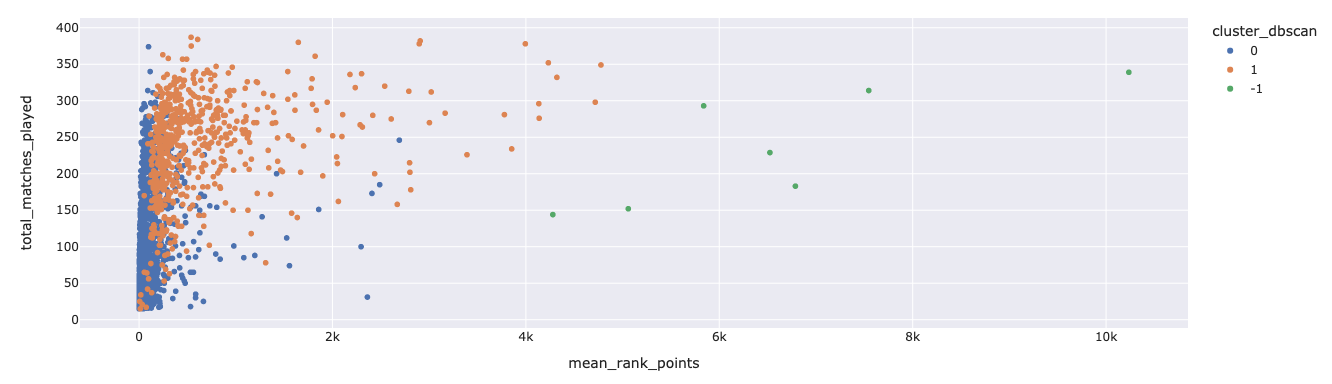
\includegraphics[width=\textwidth]{plots/dbscan/dbscan_scatter.png}
		\captionof{figure}{Results of DBSCAN}
		\label{fig:dbscan_scatter}
	\end{minipage}
\end{figure}
\begin{itemize}
    \item \textbf{Cluster 0} represents the \textbf{average Joe} (80.08\%). They have an average rank points of $72$, and the average number of matches played is $81$. Their trend of growth is slightly increasing, with a value of $1.14$.
    \item \textbf{Cluster 1} represents the \textbf{good players} (19.68\%). They have an average rank point of $658$, and fairly experienced with an average number of matches played that is $237$. Their trend of growth is increasing, with a value of $1.54$.
    \item \textbf{Outliers} are the \textbf{Gods of tennis} (0.23\%), such as Novak Djokovic, Rafael Nadal, Roger Federer, Simona Halep, Serena Williams. They have an outstanding average rank points of $6609$ and an average age of $29$ years (the average is 22 years old)! It's interesting to see that their average number of matches played is the same as Cluster 1, so the experience is the same. Moreover, their average trend of growth is decreasing with a value of $0,71$.
\end{itemize}	


% \begin{figure}[h]
% 	\centering
% 	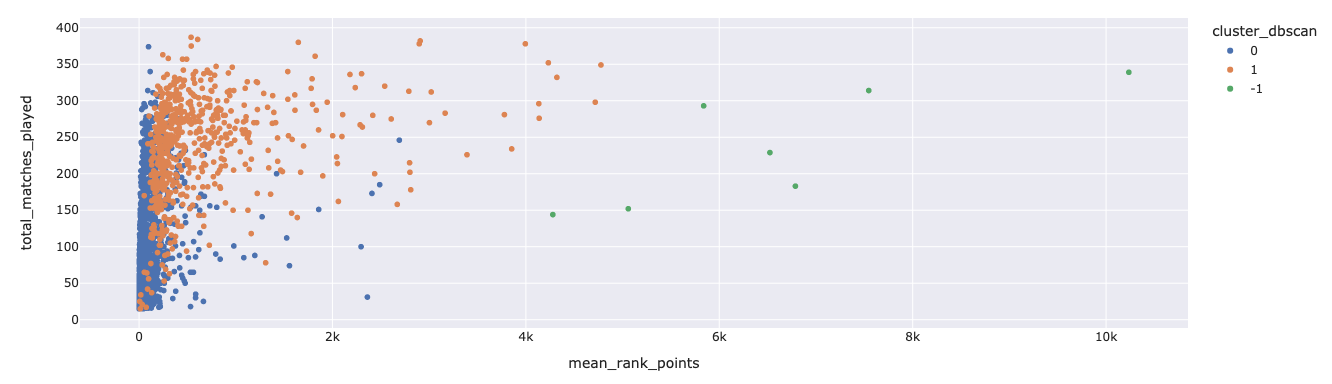
\includegraphics[width=\textwidth]{plots/dbscan/dbscan_scatter}
% 	\captionof{figure}{Results of DBSCAN}
% 	\label{fig:dbscan_scatter}
% \end{figure}

% \begin{figure}[h]
% 	\centering
% 	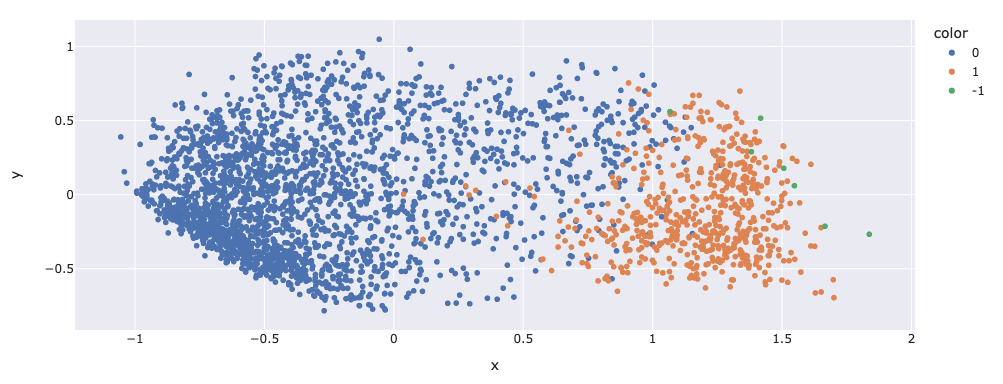
\includegraphics[width=\textwidth]{plots/dbscan/dbscan_pca.png}
% 	\captionof{figure}{PCA visualization}
% 	\label{fig:dbscan_pca}
% \end{figure}

\subsection{Hierarchical}
\label{sec:hierarchical}
The set of feature used for DBSCAN is the same as K-means, as well as for the applied transformations.\\
The agglomerative hierarchical clustering was executed with Euclidean distance and with different linkage method for the inter-cluster similarity such as \textbf{Ward}, \textbf{Complete}, \textbf{Single} and \textbf{Average}. The corresponding representation is shown in the graphs in Figure \ref{figure:hierarchical_dendrograms}, which only shows the last 9 merges.
The number of clusters was chosen based on the Silhouette score and by trying to achieve a reasonable number of clusters: between 2 and 6. We also used the dendrogram as a proxy to study the similarity between various clusters with respect to a fixed \textit{n\_clusters} parameter.\\

\subsubsection{Results interpretation}
As we could expect, Max shows greater distances with respect to Min, while Average falls in between. This is obviously due to how the different distances are computed.\\
Regarding the qualitative results shown in Table \ref{tab:hierarchical-table}, we can see how the \textit{Average} method results the best both in terms of Silhouette score both in terms of homogeneity among the cluster's size. The \textit{Single} method, on the other hand, performs the worst in terms of homogeneity and in terms of Silhouette score and by increasing the number of clusters, the results were a high number of singletons. In general, for the other methods, increasing the number of clusters led to a situation where the clustering tended to deteriorate in terms of silhouette metrics, as can be seen in the table.\\
So taking the \textbf{Average method} with 2 clusters as a reference, the results can be interpreted as follows:
\begin{itemize}
	\item{ \textbf{Cluster 0} represents the \textbf{good players} (30.36\%): those with an average rank points of 577.62 and fairly experienced with an average number of matches played that is 201.26.}
	\item{ \textbf{Cluster 1} represent the \textbf{bad players} (69.63\%): those with an average rank points of 40.30 and with a low amount of experience that is an average number of matches played that is 73.31.}
\end{itemize}
\begin{figure}[h!]
	\centering
	\begin{minipage}{.50\textwidth}
		\centering
		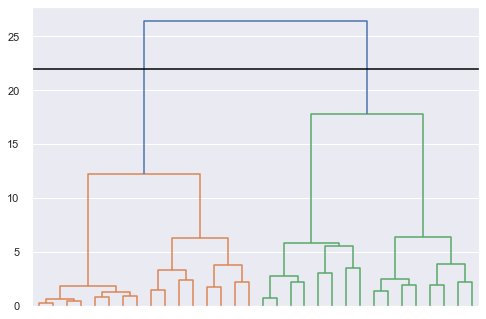
\includegraphics[width=\textwidth]{plots/hierarchical/hierarchical_dendogram_ward.png}
		\subcaptionof{(a) Ward}
	\end{minipage}%
	\begin{minipage}{.50\textwidth}
		\centering
		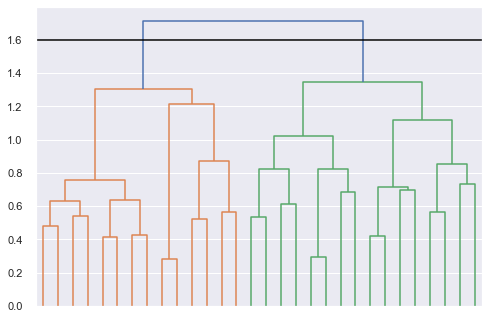
\includegraphics[width=\textwidth]{plots/hierarchical/hierarchical_dendogram_complete.png}
		\subcaptionof{(b) Complete/Max}
	\end{minipage}
	\begin{minipage}{.50\textwidth}
		\centering
		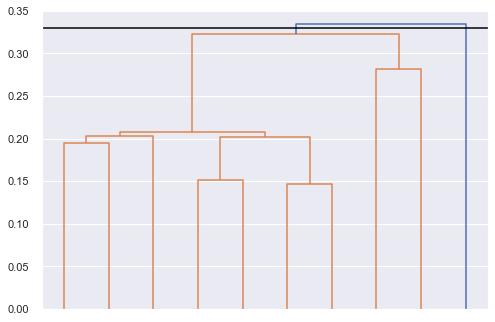
\includegraphics[width=\textwidth]{plots/hierarchical/hierarchical_dendogram_single.png}
		\subcaptionof{(c) Single/Min}
	\end{minipage}%
	\begin{minipage}{.50\textwidth}
		\centering
		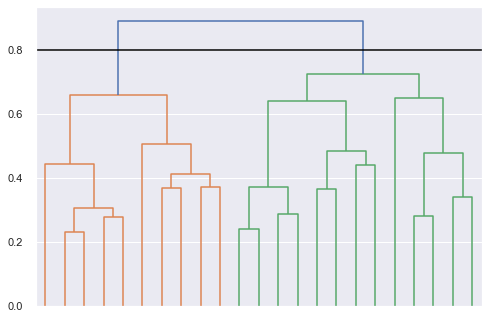
\includegraphics[width=\textwidth]{plots/hierarchical/hierarchical_dendogram_average.png}
		\subcaptionof{(d) Average}
	\end{minipage}
	\captionof{figure}{Dendrograms for hierarchical clustering}
	\label{figure:hierarchical_dendrograms}
\end{figure}

\begin{table}[h!]
\centering
\begin{tabular}{|l|l|l|l|}
\hline
\textbf{Linkage} & \textbf{K} & \textbf{Clusters'size} & \textbf{Silhouette} \\ \hline\hline
Average          & 2          & 2062, 935              & 0,482               \\ \hline
Ward             & 2          & 2110, 887              & 0,476               \\ \hline
Ward             & 4          & 1338, 772, 541, 346    & 0,467               \\ \hline
Complete         & 2          & 2333, 664              & 0,463               \\ \hline
Single           & 2          & 2996, 1                & 0,444               \\ \hline
Average          & 4          & 1545,  924,  517, 11   & 0,421               \\ \hline
\end{tabular}
\caption{Comparison between different linkage method ordered by Silhouette score}
\label{tab:hierarchical-table}
\end{table}

\subsection{Comparison}
After experimenting with the different clustering algorithms, we can draw conclusions by referring to the results obtained, which are shown in Table \ref{tab:clustering-comparison-table}.
\begin{itemize}
	\item{ \textbf{K-means} identifies 4 fairly uniform clusters and manages to describe both weak and strong players. And for both, it identifies those that are going up and those that are going down in terms of performance. It also manages to achieve the highest Silhouette score compared to the other proposed methods.}
	\item{ \textbf{DBSCAN} is the one that identifies and describes in a better way the players that are excellent at tennis, and in more general term is really good at identifying players outside the norm. At the same time, it's not great at clustering players into multiple groups that are acceptably balanced.}
	\item{\textbf{Hierarchical} the clustering results is fairly similar to the K-means both with 2 and 4 number of clusters, however in either cases it results in a lower Silhouette score.
	}
\end{itemize}
In conclusion, the algorithm that best describes the types of players within the dataset is K-means.
\begin{table}[h]
\centering
\begin{tabular}{|l|l|l|l|}
\hline
\textbf{Algorithm}     & \textbf{K} & \textbf{Clusters'size} & \textbf{Silhouette} \\ \hline
K-means                & 4          & 1350, 764, 474, 409    & \textbf{0.513}      \\ \hline
DBSCAN                 & 2          & 2400, 590, (7)         & 0,476               \\ \hline
Hierarchical (Average) & 2          & 2087, 910              & 0,486               \\ \hline
Hierarchical (Ward)    & 4          & 1338, 772, 541, 346    & 0,467               \\ \hline
\end{tabular}
\caption{Comparison between the different clustering algorithms}
\label{tab:clustering-comparison-table}
\end{table}

\subsection{Other algorithms}
In addition to the algorithms analysed above, we have also experimented with other algorithms available in the PyClustering library. 

\subsubsection{Fuzzy C-Means}
The first was C-means which is a fuzzy algorithm, in other words it is soft clustering. The algorithm was initialized with k++ initializer to find the centroids, and then we played with the parameter indicating how fuzzy the results should be, first setting $m=1.5$ and then $m=2$. In the first case, the results were almost identical to k-means (Sec. \ref{sec:k-means}), in the second case they deviated slightly, with small variations in cluster size, but the average remained particularly robust, in other words our interpretation of the clusters remained practically unchanged. Moreover, the Silhouette score decreased from $0.513$ to $0.512$.

\subsubsection{Expectation Maximization Algorithm (EMA)}
The algorithm was first used with the aim of finding a number of clusters of 4, but from a semantic point of view the results were not very different from those obtained in k-means, but the Silhouette score was much lower, so from a qualitative point of view we discarded this one. Then we tried a number of clusters equal to 2, thus obtaining the first with 1989 elements, the second with 1008 and a Silhouette of 0.458. A visualization of the result can be appreciated in the PCA reported in Figure \ref{fig:ema_pca}. The interpretation that can be given is the same as that defined for the hierarchical (Sec. \ref{sec:hierarchical}), but all in all with a lower Silhouette.
\begin{figure}[h]
	\centering
	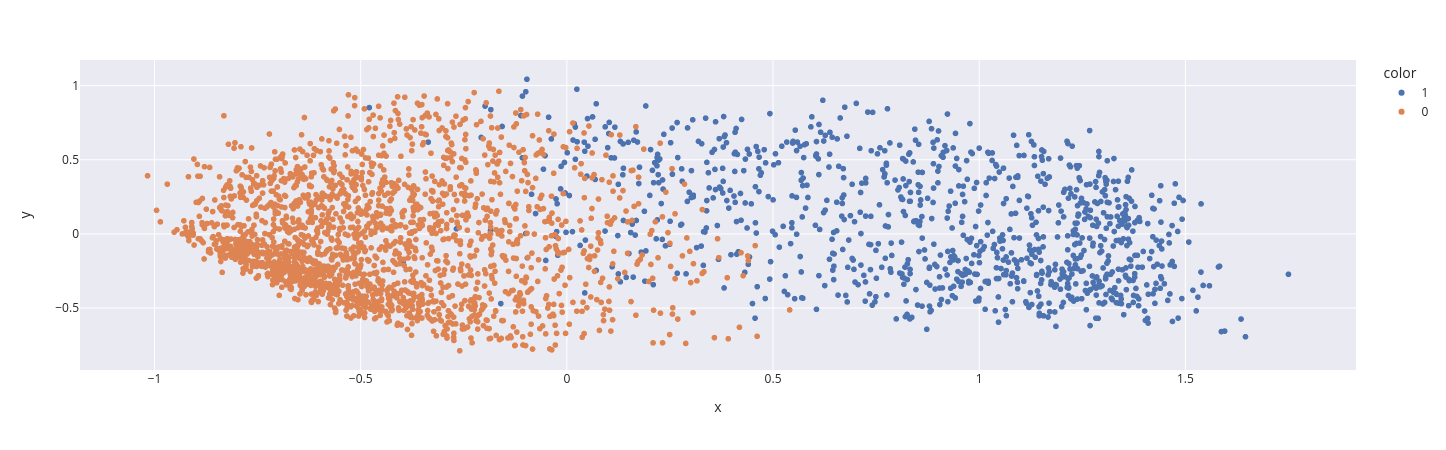
\includegraphics[width=\textwidth]{plots/ema/ema_pca.png}
	\captionof{figure}{Principal component analysis for EMA}
	\label{fig:ema_pca}
\end{figure}

\subsubsection{X-means}
Another trail we made was with X-means. We initialised the centroids with k++ initializer and set a maximum number of clusters of $40$ with the BIC algorithm performing the bisection. The results varied greatly, and often the number of clusters was particularly high or even the maximum. So the results are not interpretable, most probably due to the fact that the distribution of the data is not globular.